\section{Introduction}
\label{sec:intro}

Data exploration is the act of querying a database to discover its content.
Ultimately, the aim is to discover \emph{nuggets}, i.e., interesting queries
that expose unexpected properties of the world.  Because this task
is important and omnipresent, several engineers have devised \emph{exploration
systems} to support it. These systems let users ``play'' with their data. They
provide facilities to write queries and visualize their results quickly.
They engage their users in a loop of trials and errors, through which discover
their data. Examples of such systems are Tableau~\cite{StolteTangHanrahan2002},
based on visualizations, Blink~\cite{agarwal2012blink}, based on sampling, or
Blaeu~\cite{sellamTKDE} based on cluster analysis.

Exploration systems assume that users can evaluate the usefulness of a set of
tuples simply by looking at it. Typically, they present the results of the
queries with tables or visualizations, in the hope that users will know what to
inspect and where to go next. And indeed, this assumption holds with low
dimensionality data. If a set of tuples involves less than a dozen columns, the
users can plot it, build a mental picture of what it contains and judge whether
they effectively found a nugget or not. But the assumption breaks down in high
dimension spaces. If the data contains dozens or hundreds of columns, where
should the users look? In many cases, the query results will overwhelm them.
If the tuples contain the nugget they had been wishing for, they will
probably not be able identify it. In short, the perception of the query results becomes
a critical bottleneck in the data exploration process.

One approach to solve this problem is dimensionality reduction methods, such as
PCA. But these algorithms ignore the users' selection, hence they may miss
interesting aspects of the data. Furthermore, they transform the data: they
rescale it, project it and rotate it.  Therefore, the tuples that the users
visualize are not those that they requested in the first place. Another
approach is to use dedicated multidimensional visualization methods, such as
scatter-plot matrices or parallel coordinates. But these methods cannot scale
to the volumes we envision. For example scatter plot matrix would require at
least 190 plots to represent a simple dataset with only 20 columns. This
solution is not practical.

In this demo proposal, we introduce Ziggy, a system to help explorers
understand the results of their queries.  Ziggy detects and plots \emph{characteristic
views}, that is, small, non redundant sets of columns on which the user's
selection is different from the rest of the data. By consulting these views,
our explorers can understand what makes their tuples ``special'', and steer
their exploration accordingly.

Ziggy can detect characteristic views, but it can also justify them. For each
view, it generates a short paragraph in which it motivates its choices, using
high-level statistical properties of the data.  While several previously
published work has presented mechanisms to query databases in natural language,
little to none of them have tackled the reverse direction: how to describe
results in plain English. Our demonstration pioneers this field.

Our demo is based on two contributions, presented in a research paper currently
under submission. First, we introduce and formalize the problem of \emph{tuple
characterization}, which to our knowledge had never been studied before.
Second, we present Ziggy, our fully functional tuple description engine. Ziggy
can detect views, validate them and it can justify its choices. It can readily
be embedded in a data exploration engine.

\section{Characterizing Tuples}
\label{sec:overview}

Let us present Ziggy with an example. An analysts wants to understand what
causes violent crimes in US cities. She has access a large table, containing
130 economic, social and demographic indicators for a few thousand cities. To
seed the exploration, she selects the cities with the highest rates of
criminality. Her database front-end returns one large table with more than a
hundred columns. Which columns should she inspect?

\begin{figure}[t!]
    \centering
    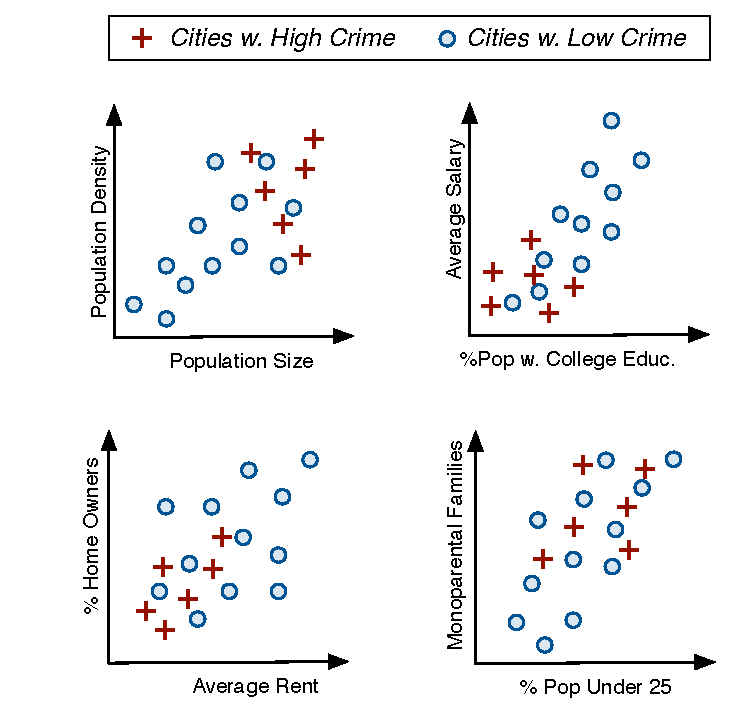
\includegraphics[width=.9\columnwidth]{Images/CharacViews}
    \caption{Four examples of characteristic views.}
    \label{fig:characteristic-views}
\end{figure}

Ziggy has two aims. First, it presents several low-dimension views of the
database, which highlight the differences between the selected tuples and the
others.  Figure~\ref{fig:characteristic-views} depicts four of those. On all
four views, we observe that the selection has an unusual statistical
distribution compared to the rest of the data. In the first plot, we see that
cities with high crime tend to have particularly high densities and number of
inhabitants. The second view shows that these cities correspond to lowest
levels of education.  The third view reveals that dangerous neighbourhoods tend
to have lower rents and a lower percentage of home ownership. The last one
reveals that they are generally younger, with more mono-parental families.


Ziggy's second aim is to \emph{explain} its choices. Indeed, our system can
veritably motivate its decisions, using natural language. For instance, it
would comment the first view of Figure~\ref{fig:characteristic-views} as
follows:
\begin{quotation}
    ``On columns~\texttt{Population} and \texttt{Density}, your selection has
    particularly high values and a low variance''
\end{quotation} 
This short paragraph describes why Ziggy chose the columns \texttt{Population}
and \texttt{Density}. The users can use these explanations as a hint for further
exploration. Thus, they make sure that they have not missed any potentially
interesting aspect of the data. Alternatively, they can use it for sanity
checks, to control the correctness of Ziggy's views.

\section{Problem Formulation}
\label{sec:algorithm}

We gave an intuitive overview characteristic views and we explained why they
were useful. We now formalize this concept. First, we will present Ziggy's
underlying objective function in its general form. Then we will describe in
more detail how Ziggy computes the ``peculiarity'' of a view.

\subsection{General Statement} 
When seeking views, Ziggy must consider two
aspects. First, it must find columns on which the users' selection behaves
unusually. Second, it must enforce that its views are not redundant with each
other. Let us formalize these objectives.

\label{sec:problem}
\begin{figure}[t!]
    \centering
    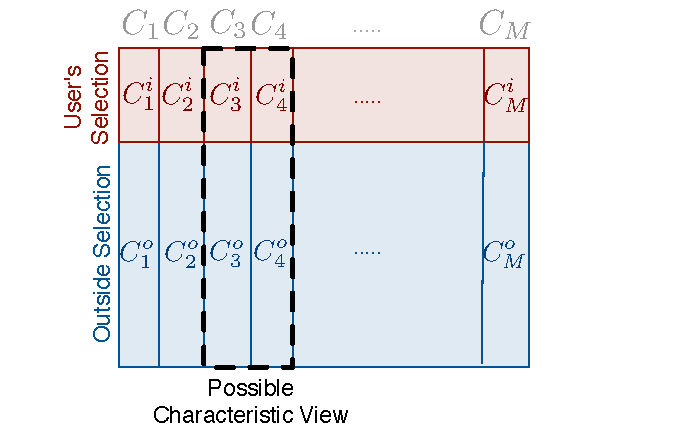
\includegraphics[width=0.6\columnwidth]{Images/Setting}
    \caption{Our problem setting.}
    \label{fig:setting}
\end{figure}
To measure the selection's unusualness, Ziggy exploits differences in
statistical distributions between the selected tuples and the rest of the
database. Let the random variables $C_1, \ldots, C_M$ represent the $M$ columns
in the database.  We assume that the variable $C_j^i$ represent the tuples
inside the selection, and that $C_j^o$ represent the tuples outside the
selection, as shown in Figure~\ref{fig:setting}. Ziggy's aim is to find a set
of at most $D$ columns such that the distribution of $C_1^o, \ldots, C_D^o$ is
as different as possible from that of $C_1^i, \ldots, C_D^i$. If $\mathfrak{D}$
represents a measure of statistical divergence from the statistics literature,
our aim is to find the top views $\mathcal{V}_i = \{C_1, \ldots, C_D\}$ that
maximize the following quantity:
\begin{equation}
    \label{eq:objective0}
        \mathfrak{D}\big( C_1^o, \ldots, C_D^o \,;\, C_1^i, \ldots, C_D^i \big)\\
\end{equation}
Common examples of divergence functions $\mathfrak{D}$ are the distance between
the centroids and the Kullback-Leibler divergence~\cite{wasserman2013all}.  We
will present our own in the next subsection.

Equation~\ref{eq:objective0} is not complete because it can lead to
redundancy: a small number of columns may appear in all the best views. To
tackle this effect, we introduce a constraint in our problem statement.  Assume
that we have already discovered $i-1$ views $\mathcal{V}_1, \ldots,
\mathcal{V}_{i-1}$. Let the notation $\mathcal{V}_{1 \ldots i-1}$ describe
their union, i.e., $\mathcal{V}_{1 \ldots i-1} = \bigcup_{v \in [1,i-1]}
\mathcal{V}_v$. For some user-defined integer $L$, our aim is to find a new
view $\mathcal{V}_i$ that solves the following optimization problem:
\begin{equation}
    \label{eq:objective}
    \begin{aligned}
        \text{Argmax}_{\mathcal{V}_i =\{C_1, \ldots, C_D\}}\; 
        & \mathfrak{D}\big( C_1^o, \ldots, C_D^o \,;\, C_1^i, \ldots, C_D^i \big)\\
         \text{s.t.} 
         & \left|  \mathcal{V}_i \cap \mathcal{V}_{1\ldots i-1}\right|  <L\\ 
    \end{aligned}
\end{equation}
The constraint enforces view diversity: it makes sure that that the new view
$\mathcal{V}_i$ uses less than $L$ columns from the precedent views.

\subsection{Dissimilarity Measure}
The statistics literature presents many options to instantiate the statistical 
divergence measure $\mathfrak{D}$~\cite{wasserman2013all}. But most of those
operate in a ``black box'' fashion: they indicate how much two distributions
differ, but they do not explain why. We now introduce our own function, the
\emph{Zig-Dissimilarity}, that overcomes this problem.

\begin{figure}[t!]
    \centering
    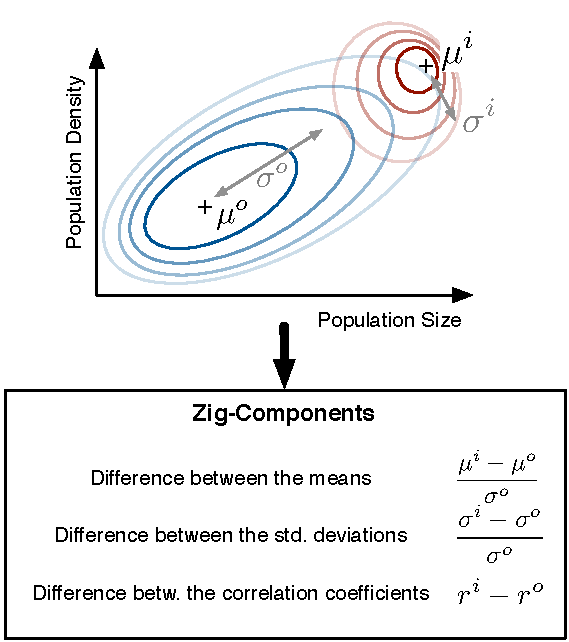
\includegraphics[width=.7\columnwidth]{Images/Zig-Dissimilarity}
    \caption{Examples of Zig-Components.}
    \label{fig:zig-dissim}
\end{figure}

The main idea behind the Zig-Dissimilarity is to  compute several simple
indicators of dissimilarity, the \emph{Zig-Components}, and aggregate them into
one synthetic score.  Figure~\ref{fig:zig-dissim} presents three such
indicators: the difference between the means, the difference between the
standard deviations and the difference between the correlation coefficients. We
see that each Zig-Component highlights one particular ``aspect'' of the
difference between the distributions.  Also, these functions are verifiable:
the users can inspect the charts and check whether they hold.  Most of our
Zig-Components come from the statistics literature, where they are referred to
as \emph{effect sizes}~\cite{hedges2014statistical}. Observe that we test
dissimilarities in spaces with one or two dimension. For instance, the difference
between the correlation coefficients involves two dimensions. In principle, we
could design Zig-Components for higher dimensionalities.  Nevertheless,
experience revealed that those add significant processing times for minimal
gains in accuracy.  Also, we ignore the components related to categorical data
for now - we discuss them in our full paper.

To aggregate the Zig-Components, we compute their absolute value, normalize
them and compute a weighted sum.  The normalization enforces that the
indicators have comparable scale. The weights in the final sum are defined by
the user. Thus, they can express their preference for one type of difference
over the others. 

\section{Ziggy's Architecture}
\label{sec:solution}


We formalized the multi-view characterization problem. We now present how Ziggy
solves it.

Figure~\ref{fig:architecture} presents Ziggy's tuples description pipeline.  It
includes three stages: preparation, view construction and post-processing.
During the preparation stage, Ziggy collects the statistics necessary to build
the views. In the View Construction stage, it effectively forms the views,
i.e., the groups of columns. During the last step, it checks if the views are
statistically robust and it generates the justifications.
\begin{figure}[t!]
    \centering
    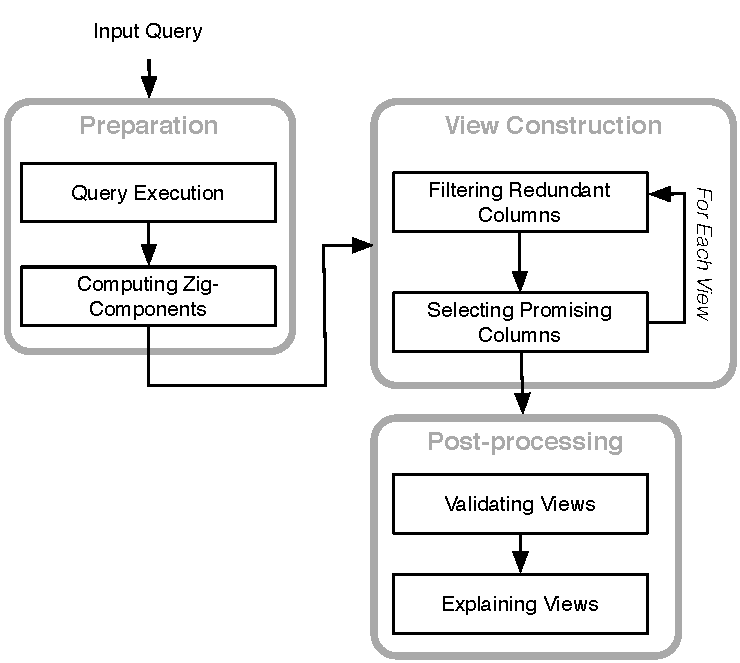
\includegraphics[width=\columnwidth]{Images/Algorithm}
    \caption{Ziggy's Tuples Description Pipeline.}
    \label{fig:architecture}
\end{figure}

\textbf{Preparation.} During the preparation step, Ziggy executes the user's
query and it computes the Zig-Components associated to each column and each
couple of columns in the results. This step is by far the most time consuming.
In our manuscript, we present a strategy to share computations between queries,
and therefore reduce the amount of data to read. The output of this step is a
table, which describes the Zig-Components associated to each variable and each
pair of variables.

\textbf{View Construction.} In this step, Ziggy builds the views one by one, in
a greedy manner. At the beginning of each iteration, it detects the columns
that violate the redundancy constraint of Equation~\ref{eq:objective} and
discards them. Then, it detects the pairs of columns associated to the highest
Zig-Dissimilarities, and it appends them one by one to the view. It stops when
all the columns are included in at least one view, or when the differences are
too weak for the results to be statistically significant (cf. next step).

\textbf{Post-Processing.} During the post-processing phase, Ziggy evaluates the
statistical robustness of the views. The aim is to control spurious findings,
that is, differences caused by chance alone. For each view, it tests the
significance of the Zig-Component separately, using asymptotic bounds from the
literature~\cite{hedges2014statistical}. Then it aggregates the confidence
scores associated to each component. Depending on the users' preferences, it
retains the smallest value, or it uses more advanced aggregation schemes such
as the Bonferroni correction~\cite{wasserman2013all}. 

During the last step, Ziggy also generates the explanations. Given the
composite nature of the Zig-Dissimilarity, this step is straightforward: Ziggy
choses the Zig-Components associated with the highest level of confidence, and
it describes them with text. We implemented text generation and rewriting
with hand-written rules.


\section{Implementation and Demo}
\label{sec:demo}

\begin{figure*}[t!]
    \centering
    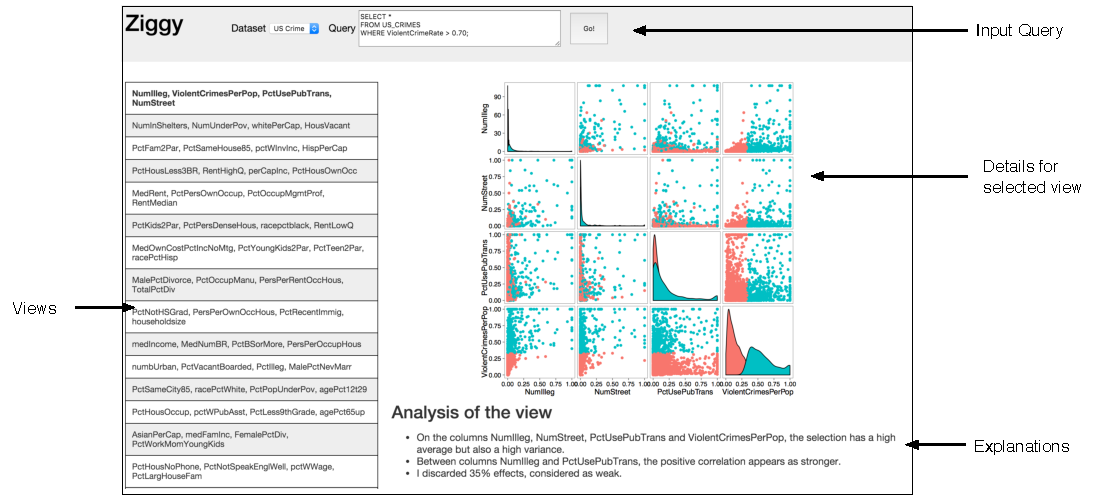
\includegraphics[width=\textwidth]{Images/ScreenDetail}
    \caption{Snapshot of Ziggy's interface.}
    \label{fig:screenshot}
\end{figure*}

\subsection{Overview of the System}
\label{sec:archi}
Our demonstration system comprises three components. In the bottom layer, a
DBMS stores and delivers the data (we chose MonetDB). The middle layer
comprises the tuple characterization engine and a Web server. We developed both
components with the statistical language R, except for a few critical
operations written in C (those related to computing Zig-Components). The Web
server relies on the package \texttt{Shiny}. The front end is based on a
HTML/Javascript application. 

Figure~\ref{fig:screenshot} presents a screenshot of our demonstration system.
Users specify their queries in the text box of the top panel. Ziggy returns the
views on the left side, and the explanations on the right side.

\subsection{Use Cases}
\label{sec:usecases}

We will demonstrate Ziggy with three real-life datasets, presented in
increasing order of complexity.
\begin{itemize}
    \item The \textbf{Box Office} dataset describes Hollywood movies released
        between 2007 and 2013. We will use it to introduce the main concepts behind
        Ziggy: the tuple description problem, how Ziggy choses views and how to
        read them. The data contains 900 tuples and 12 columns.
    \item The \textbf{US Crime} database contains 128 crime and socio-economic
        indicators for 1994 US Cities. The dataset is freely available on the
        UCI Repository\footnote{\url{https://archive.ics.uci.edu/ml/datasets/Communities+and+Crime}}.
        The use case is similar to the running example used throughout this
        paper. We hope to surprise our visitors by showing that seemingly
        unrelated variables can have a strong predictive power - such as the
        number of boarded windows in a given neighborhood.
    \item The \textbf{Countries and Innovation} dataset describes innovation
        and patents for different regions of the world. We obtained it by
        combining different tables from the Website of the OECD, an international
        economic organization\footnote{\url{http://stats.oecd.org/}}. It
        contains 6,823 rows and 519 columns. We will show that Ziggy can
        highlight complex phenomena, in effect generating hypotheses for future
        exploration.
\end{itemize}
During our presentation, we will use ready-made queries and encourage the
visitors to suggest their own.

\section{Conclusion}
\label{sec:conclusion}
During the last few years, authors have introduced dozens of methods to
discover new, interesting queries. In this paper, we tackled the complementary
problem: once our users have a query, how do they know if it is a good one?
Our short term objective to demonstrate Ziggy and let visitors challenge our
system. On the long term, we intend to distribute our tuples description engine
as a library, to be included into external exploration systems.
